\scanpage{120}
\mspage{5}

On a donc trouvé $4=1+3$ présentations du groupoïde fondamental $\Pi_1(\widetilde{X}^{\substack{*\\*}*},S)$, suivant qu'on utilise tous les chemins $(8)$, $(9)$, ou qu'on élimine les chemins $a_r^i$ \inserted{($i$ fixé), dans l'exemple $i=1$)} et les sommets qui se trouvent dessus. Je vais maintenant examiner le cas où on élimine $=$ deux côtés du triangle fondamental i.e. où on ne garde les $a_r^i$ que d'un seul type --- disons les $a_r^\infty$ --- ce qui conduit aussi : éliminer tous les sommets proches des $R_\varphi$ \inserted{($\varphi\in S$)} de type \deleted{infini} \inserted{$\infty$ et ceux qui leur sont reliés}, \deleted{\unsure{enfin}, des centres des faces} \inserted{etc.} --- i.e. \deleted{les $R_r^i$} à ne garder que les $R_r^{ij}$ avec \deleted{\unsure{pour}} \inserted{$(i,j)\in\{0,1\}$} \deleted{$\unsure{i,j\ne\infty}$, \unsure{les côtés ne passent pas par $\infty$})} :

\noindent\begin{minipage}[c]{.54\linewidth}
\[
(17)\qquad R_r^{i,j}\quad\left\{\begin{array}{l}
r\in\mathcal{R}\\
\{i,j\}=\{0,1\}
\end{array}\right.
\]
\end{minipage}\hfill
\begin{minipage}[c]{.43\linewidth}
\begin{tikzpicture}[x=1cm,y=1cm]
\node[anchor=west,inner sep=0pt,font=\scriptsize] at (.18,0) {$\left\{\begin{aligned}
R_r^{0,1}&=R_{\tau_\infty r}^{0,1},\\
R_r^{1,0}&=Q_{\tau_\infty(r)}
\end{aligned}\right.$};
\draw[line width=.4pt] (-.05,.65)--(2.5,.8) (-.05,.5)--(-.05,-.65) (.1,-.75)--(4,-.65);
\node[anchor=west,inner sep=0pt,text width=.95cm,font=\scriptsize] at (3.2,.25) {pour mémoire};
\node[anchor=north,inner sep=0pt,text width=2.5cm,align=center,font=\scriptsize] at (2,-.86) {relations de redondance};
\end{tikzpicture}
\end{minipage}

\[
(18)\qquad\left\{\begin{aligned}
a_r^\infty &: \unsure{R_r^{01}|R_r^{0,1}}\underset{\longrightarrow}{\deleted{\unsure{\to R}}}R_r^{1,0} \qquad(\forall r\in\mathcal{R})\\
\Lambda_r^0\unsure{,}\deleted{\unsure{\Lambda_r^{\prime1}|\Lambda_r^1}} &:R_r^{01}\longrightarrow\unsure{R_{\tau_1(r)}^{01}|R_{\tau_1r}^{01},}\\
\Lambda_r^{\prime1} &:R_r^{10}\longrightarrow\unsure{R_{\tau_0(r)}^{1,0}|R_{\tau_0r}^{1,0},}
\end{aligned}\right.
\]

\noindent\begin{minipage}[t]{.48\linewidth}
\vspace{0pt}
\figure{
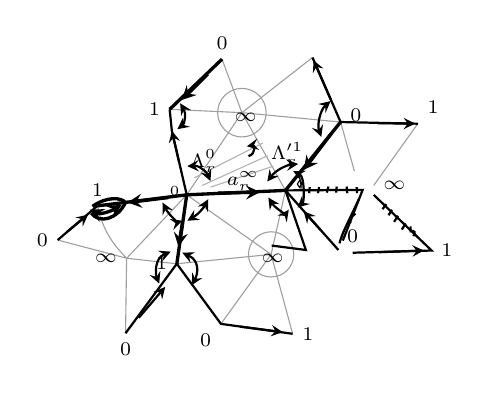
\begin{tikzpicture}[x=.007cm,y=-.007cm,>=stealth,font=\scriptsize]
% Pale triangular construction routes and the two drawn circular contours.
\draw[gray!75] (247,1588)--(378,1594)--(557,1611)
  (342,1497)--(378,1594)--(457,1735)--(278,1743)--(378,1594)--(506,1494);
\draw[gray!75] (116,1763)..controls(128,1817)and(153,1841)..(169,1858)
  (44,1825)--(169,1858)--(167,1994) (169,1858)--(260,1868)
  (169,1858)--(278,1743)--(431,1851)--(260,1868);
\draw[gray!75] (457,1735)--(431,1851)--(340,1977)
  (431,1851)--(470,1995) (557,1611)--(582,1700) (617,1726)--(697,1614);
\draw[gray!75] (378,1594) circle (44) (431,1851) circle (41);
\draw[gray!60] (292,1712)--(416,1649) (306,1726)--(425,1672) (321,1729)--(435,1691);
% Upper left and upper right boundaries; heads lie along the full contours.
\draw[very thick] (342,1497)--(247,1588);
\draw[very thick,->] (316,1524)--(269,1571);
\draw[thick] (278,1743)--(251,1627)--(247,1588);
\draw[thick,->] (264,1683)--(251,1627);
\draw[thick,<->] (266,1577)..controls(277,1595)and(274,1614)..(261,1624);
\draw[thick] (557,1611)--(506,1494);
\draw[thick,->] (539,1570)--(508,1499);
\draw[thick,<->] (539,1573)..controls(521,1588)and(514,1615)..(522,1638);
\draw[thick] (557,1611)--(697,1614);
\draw[thick,->] (624,1613)--(692,1614);
\draw[very thick] (557,1611)--(457,1735);
\draw[very thick,->] (540,1632)--(490,1698);
% The three full dark routes from the central-left junction.
\draw[very thick] (278,1743)--(457,1735);
\draw[very thick,->] (334,1740)--(411,1738);
\draw[very thick] (278,1743)--(260,1868);
\draw[very thick,->] (270,1795)--(263,1837);
\draw[very thick] (278,1743)--(116,1763);
\draw[very thick,->] (244,1748)--(171,1757);
\draw[thick,<->] (279,1691)..controls(305,1690)and(316,1706)..(321,1718);
\draw[thick,<->] (424,1719)..controls(440,1698)and(459,1689)..(480,1687);
\draw[thick,<->] (234,1757)..controls(247,1782)and(264,1792)..(270,1790);
\draw[thick,<->] (279,1790)..controls(301,1777)and(310,1764)..(317,1751);
% Southeast contours: the outer ray points back toward the central junction.
\draw[thick] (457,1735)--(494,1843)--(432,1835);
\draw[thick] (457,1735)--(553,1843);
\draw[thick,->] (521,1807)--(490,1773);
\draw[thick,<->] (471,1700)..controls(492,1710)and(491,1755)..(479,1766);
\draw[thick,<->] (426,1748)..controls(439,1768)and(458,1777)..(463,1770);
% Hatched right-hand routes, preserving the doubled oblique trace.
\draw[thick] (457,1735)--(597,1734)--(561,1826);
\draw[thick] (590,1751)..controls(575,1784)and(559,1813)..(555,1831);
\draw[thick] (501,1729)--(500,1740) (518,1729)--(516,1740)
  (535,1728)--(532,1739) (550,1728)--(549,1739)
  (568,1728)--(569,1740) (586,1729)--(587,1740);
\draw[thick] (584,1777)--(577,1783) (576,1791)--(569,1797);
\draw[thick] (617,1743)--(722,1844)--(579,1848);
\draw[thick,->] (627,1847)--(708,1844);
\draw[thick] (640,1760)--(633,1769) (650,1770)--(644,1780)
  (661,1781)--(654,1792) (675,1795)--(668,1806);
\draw[thick] (684,1800)--(684,1809)..controls(691,1807)and(694,1811)..(689,1818);
% Lower fan and its two opposed corner arcs.
\draw[thick] (167,1994)--(260,1868)--(340,1977)--(470,1995);
\draw[thick,->] (191,1966)--(239,1910);
\draw[thick,->] (375,1982)--(452,1992);
\draw[thick,<->] (249,1846)..controls(220,1858)and(221,1886)..(228,1904);
\draw[thick,<->] (270,1848)..controls(303,1863)and(297,1889)..(287,1907);
% Doubled, heavily traced small loop at the far left.
\draw[thick] (44,1825)--(116,1763);
\draw[thick,->] (61,1810)--(99,1779);
\draw[very thick,<->] (102,1770)..controls(122,1779)and(142,1772)..(160,1761);
\draw[very thick] (107,1764)..controls(134,1745)and(160,1748)..(167,1757)
  ..controls(153,1786)and(120,1797)..(105,1776);
\draw[thick,->] (390,1673)..controls(406,1667)and(398,1653)..(387,1655);
% Written labels, including the tiny central-left oval.
\node[above] at (342,1497) {$0$};\node[left] at (247,1588) {$1$};
\node at (385,1602) {$\infty$};\node[right] at (557,1599) {$0$};
\node[above right] at (697,1614) {$\unsure{1}$};
\node[right] at (617,1726) {$\infty$};
\node[above] at (579,1848) {$0$};\node[right] at (722,1844) {$1$};
\node[right] at (470,1995) {$1$};\node[below left] at (340,1977) {$0$};
\node[below] at (167,1994) {$0$};\node[left] at (260,1868) {$1$};
\node[left] at (169,1858) {$\infty$};\node[left] at (44,1825) {$0$};
\node[above] at (116,1763) {$1$};\node at (434,1858) {$\infty$};
\node[above,inner sep=.1pt] at (256,1745) {$\scriptstyle0$};
\node at (308,1682) {$\Lambda_r^0$};\node at (460,1669) {$\Lambda_r^{\prime1}$};
\node at (380,1718) {$a_r^\infty$};
\node[inner sep=0pt] at (483,1724) {$\unsure{\vcenter{\hbox{\tikz[x=1mm,y=1mm,line width=.4pt]{
  \draw (.1,.45)--(.42,.95)--(.68,.48)--(.37,.03)--(.1,.45);
  \draw (.43,.88)..controls(.72,.58)and(.44,.24)..(.56,-.12);
}}}}$};
\end{tikzpicture}
}
pavage par des \inserted{faces} polygonales de centre des sommets de type $\infty$ --- les coins de ces polygones étant arrondis pour éviter les trous
\end{minipage}\hfill
\begin{minipage}[t]{.49\linewidth}
\vspace{0pt}
\inserted{avec} relations de redondance seulement
\[
(19)\quad\boxed{\begin{aligned}
\Lambda_r^0\Lambda_{\tau_1(r)}^0&=1\\
\Lambda_r^{\prime1}\Lambda_{\tau_0(r)}^{\prime1}&=1
\end{aligned}}
\]
c'est donc directement exprimé comme un groupoïde libre. Cela fait trois autres présentations de $\Pi_1(X)$, mais sur des ens. de sommets différents, savoir $\Pi_1(\widetilde{X}^{\vcenter{\hbox{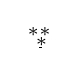
\begin{tikzpicture}[x=1mm,y=1mm]
\node[inner sep=0pt] at (0,1.5) {$\scriptstyle *$};
\node[inner sep=0pt] at (1.5,1.5) {$\scriptstyle *$};
\node[inner sep=0pt] at (1.05,.2) {$\scriptstyle *$};
\node[inner sep=0pt] at (.95,-.8) {$\unsure{\vcenter{\hbox{\tikz[x=1mm,y=1mm]{\draw[line width=.35pt] (0,0)--(.35,0);}}}}$};
\end{tikzpicture}}}},S-S_i)$, pour $i=\infty$ (cas explicité\unsure{]|)} ou $0$ ou $1$.
\end{minipage}

\mspage{119}
